%!TEX root = ../../thesis.tex

\section{Future Work: Models}
\label{sec:future-models}

Next we turn to the research directions of models for future work. We first describe the desiderata of reading comprehension models. Most of the existing work only focuses on \ti{accuracy} --- given a standard training/development/testing split of a dataset, the major goal is to get the best accuracy score on the testing set. However, we argue that there are other important aspects which have been overlooked that we will need to work on in the future, including \ti{speed and scalability}, \ti{robustness} and \ti{interpretability}. Lastly, we discuss what important elements are still missing in the current models, to solve more difficult reading comprehension problems.

\subsection{Desiderata}
Besides \ti{accuracy} (achieving a better performance score on a standard dataset), the following desiderata are also very important for future work:

\paragraph{Speed and Scalability.} How to build faster models (for both training and inference) and how to scale to longer documents is an important direction to pursue. Building faster models for training can lead to lower turnaround time for experimentation and also enable us to train on bigger datasets. Building faster models for inference is highly useful when we deploy the models in practical use. Also, it is unrealistic to encode a very long document (e.g., \sys{TriviaQA}) or even a full book (e.g., \sys{NarrativeQA}) using an RNN and this still remains a severe challenge. For example, the average document length of \sys{TriviaQA} is 2,895 tokens and the authors truncated the documents to the first 800 tokens for the sake of scalability. The average document length of \sys{NarrativeQA} is 62,528 tokens and the authors have to first retrieve a small number of relevant passages from the story using an IR system.

Existing solutions to these problems include:
\begin{itemize}
    \item
        Replacing LSTMs with non-recurrent models such as \sys{Transformer}~\cite{vaswani2017attention} or lighter recurrent units such as \sys{SRU}~\cite{lei2018simple} as we discussed in Section~\ref{sec:alt-lstms}.
    \item
        Training models which learn to skip part of the documents so they don't need to read all of the content. These models can run much faster while still retaining a similar performance. Representative works in this line include \newcite{yu2017learning} and \newcite{seo2018neural}.
    \item
        The choice of optimization algorithms can also greatly affect the convergence speed. Multi-GPU training and hardware performance are also important aspects to consider but they are beyond the scope of this thesis. \newcite{coleman2017dawnbench} provide a benchmark\footnote{\href{https://dawn.cs.stanford.edu/benchmark/}{https://dawn.cs.stanford.edu/benchmark/}} which measures the end-to-end training and inference time to achieve a state-of-the-art accuracy level for a wide range of tasks, including \sys{SQuAD}.
\end{itemize}


\paragraph{Robustness.} We discussed in Section~\ref{sec:squad-errors} that existing models are very brittle to adversarial examples which will become a severe problem when we deploy these models in the real world. Moreover, most of the current works follow the standard paradigm: training and evaluating on the splits of one dataset. It is known that if we train our models on one dataset and evaluate on another dataset, the performance will drop dramatically due to their different source of text and construction methods. For future work, we need to consider:
\begin{itemize}
    \item How to create better adversarial training examples and incorporate them into the training process.
    \item Researching more on transfer learning and multi-task learning, so that we can build models with high performance across various datasets.
    \item We might need to break the standard paradigm of supervised learning, and think about how to create better ways of evaluating our current models for the sake of building more robust models.
\end{itemize}

\paragraph{Interpretability.} The last important aspect is \ti{interpretability} and it has been mostly ignored in the current systems.  Our future systems should not only be able to provide the final answers, but also provide the rationales behind their predictions, so users can decide if they can trust the outputs and leverage them or not. Neural networks are especially notorious for the fact that the end-to-end training paradigm makes these models like a black box and it is hard to interpret their predictions. This is especially crucial if we want to apply these systems to medical or legal domains.

Interpretability can have different definitions. In our context, we think there could be several ways to approach that:
\begin{itemize}
    \item
        The easiest way is to require the models to learn to extract input pieces from the documents as supporting evidence. This has been studied before (e.g., \cite{lei2016rationalizing}) for sentence classification problems but not yet in reading comprehension problems.
    \item
        A more complex way is that the models can indeed generate rationales. Instead of only highlighting the relevant piece of information in the passage, the models need to interpret how these pieces are connected and finally get to the answer. Take Figure~\ref{fig:sar-squad-errors} (c) as an example, the systems need to interpret that the two cities are the two largest and 3.7 million is bigger than 1.3 million thus it is the second largest. We think this desiderata is very important but far beyond the scope of current models.
    \item
        Finally, another important aspect to consider is what training resources we can get to approach this level of interpretability. Inferring rationales from the final answers is feasible but quite difficult. We should consider collecting human explanations as the supervision of training rationales in the future.
\end{itemize}

\subsection{Structures and Modules}
In this section, we are going to discuss what are the missing elements in the current models, if we want to solve more difficult reading comprehension problems.

First of all, current models are all built on either sequence models or tackle all pairs of words symmetrically (e.g., \sys{Transformer}), and omit the inherent structure of language. On the one hand, this forces our models to learn all the relevant linguistic information from scratch, which makes the learning of our models more difficult. On the other hand, the NLP community has put a lot of effort into studying linguistic representation tasks (e.g., syntactic parsing, coreference) and building many linguistic resources and tools for years. Language encodes meaning in terms of hierarchical, nested structures on sequences of words. Would it be still useful to encode linguistic structures more explicitly in our reading comprehension models?

Figure~\ref{fig:corenlp-output} illustrates the \sys{CoreNLP}~\cite{manning2014stanford} output of several examples in \sys{SQuAD}. We believe that this structural information would be useful as follows:

\begin{enumerate}[(a)]
    \item
        The information that \ti{2,400} is a \ti{numeric modifier} of \ti{professors} should help answer the question \ti{What is the total number of professors, instructors, and lecturers at Harvard?} (We have seen this example as an error case in Figure~\ref{fig:sar-squad-errors}).
    \item
        The coreference information that \ti{it} refers to \ti{Harvard} should help answer the question \ti{Starting in what year has Harvard topped the Academic Rankings of World Universities?}.
\end{enumerate}

Therefore, we think that these linguistic knowledge/structures would be still a useful addition to the current models. The remaining questions that we need to answer are: 1) What are the best ways to incorporate these structures into sequence models? 2) Do we want to model the structures as a latent variable or rely on off-the-shelf linguistic tools? For the latter case, are the current tools good enough so that the models can benefit more (rather than suffering from noise)? Can we further improve the performance of these representation tasks?

\begin{figure}[t]
  \center
  (a)
  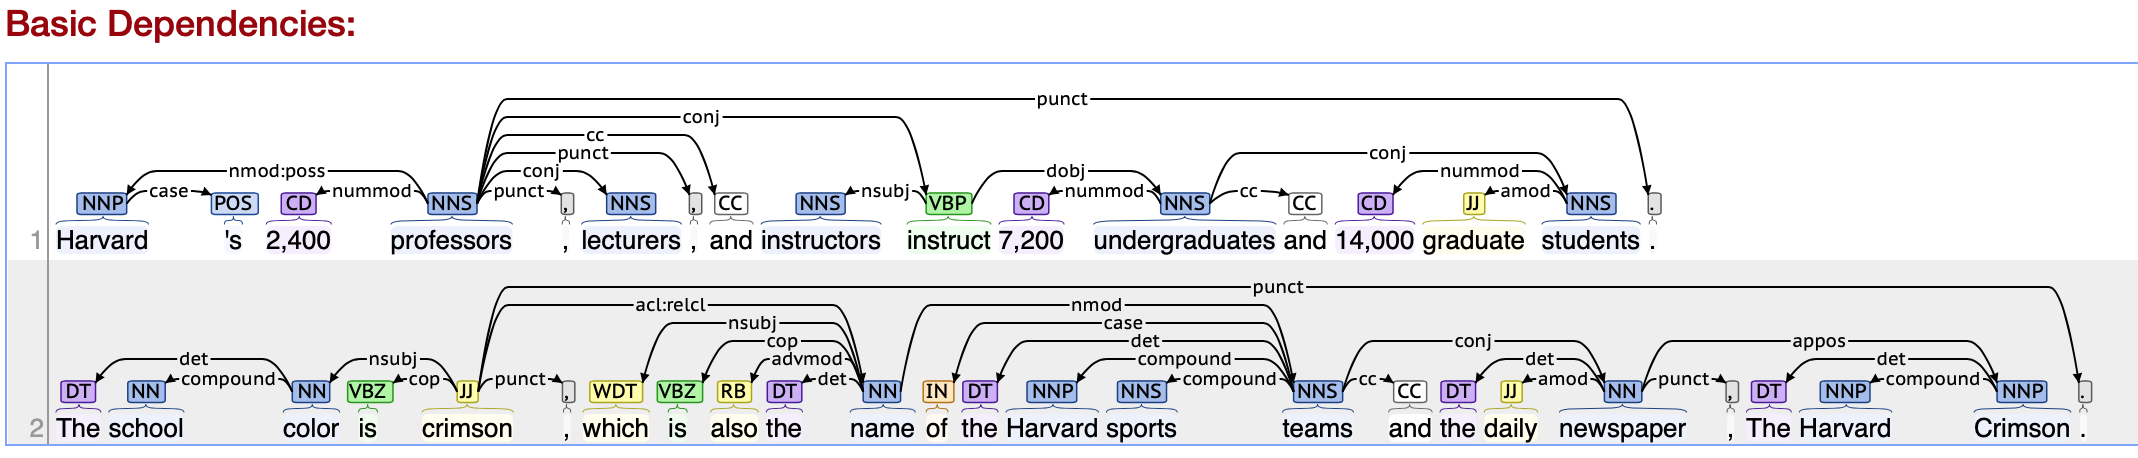
\includegraphics[scale=0.20]{img/dep_example.png}
  (b)
  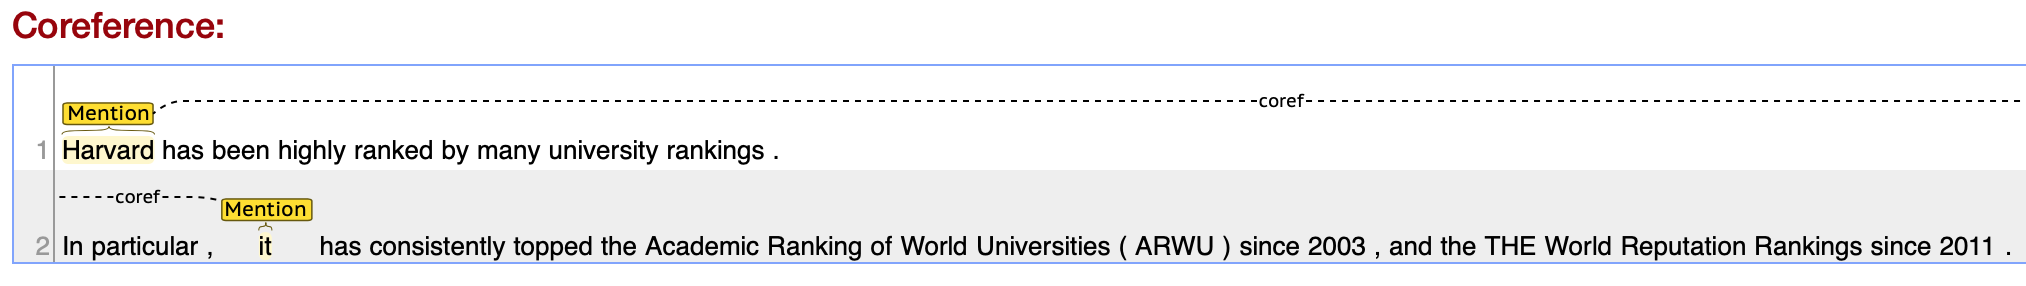
\includegraphics[scale=0.42]{img/coref_example.png}
  \longcaption{Example output of \sys{CoreNLP}: dependencies and coreference}{\label{fig:corenlp-output} Example output of \sys{CoreNLP}: (a) dependencies and (b) coreference. The image is taken from \href{http://corenlp.run}{http://corenlp.run}.}
\end{figure}

Another aspect we think is still missing from most existing models is \ti{modules}. The task of reading comprehension is inherently very complex and different types of examples require different types of reasoning capabilities. It still remains a grand challenge if we want to learn everything through a giant neural network (This is reminiscent of why the attention mechanism was proposed because we don't want to squash the meaning of a sentence or a paragraph into one vector!). We believe that, if we want to approach deeper level of reading comprehension, our future models will be more structured, more modularized, and solving one comprehensive task can be decomposed into many subproblems and we can tackle each smaller subproblem (e.g., each reasoning type) separately and combine all of them in the end.

The idea of \ti{modules} has been implemented in \sys{Neural Module Networks (NMN)} \cite{andreas2016learning} before. They first perform a dependency parse of the question, and then decompose the question answering problem into several ``modules'' based on the parse structure. One example they used for a visual question answering (VQA) task is: a question ``What color is the bird?'' can be decomposed as two modules. One module is used to detect the bird in the given image, and another module is used to detect the color of the found region (bird). We believe that this sort of approach holds promise to answer questions such as \ti{What is the population of the second largest city in California?} (Figure~\ref{fig:sar-squad-errors} (c)). However, \sys{NMN} has only been studied on visual question answering or small knowledge-base question question problems so far, and applying to reading comprehension problems can be more challenging due to the flexibility of language variations and question types.
